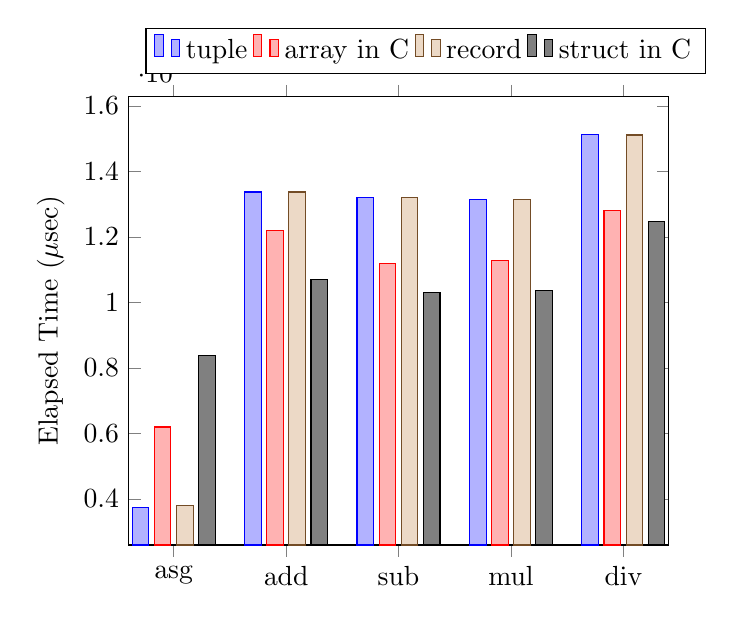
\begin{tikzpicture}
\begin{axis}[
  ybar, bar width=6pt,
  ylabel=Elapsed Time ($\mu$sec),
  symbolic x coords={asg, add, sub, mul, div},
  legend style={at={(0.55, 1.05)}, anchor=south, legend columns=4}]
\addplot coordinates
  {(asg, 3733.8) (add, 13373.6) (sub, 13202.2) (mul, 13135) (div, 15143.4)};
\addplot coordinates
  {(asg, 6198.2) (add, 12207.6) (sub, 11178) (mul, 11278.8) (div, 12806)};
\addplot coordinates
  {(asg, 3788.4) (add, 13375.2) (sub, 13210.4) (mul, 13145.2) (div, 15115.2)};
\addplot coordinates
  {(asg, 8392.8) (add, 10704.6) (sub, 10299.4) (mul, 10362.4) (div, 12472.4)};
\legend{tuple, array in C, record, struct in C}
\end{axis}
\end{tikzpicture}
